\section{Result}

We experiment our models with different thresholds and compare with constant rebalanced portfolio (CRP). 
CRP is a portfolio policy that maintain the weights thoughtout the trading period. 
Our system successfully delivers portfolios with different MDD to meet various investors' preferences, and output performed CRP in MDD and CAGR in most situations.
\begin{figure}[ht]
  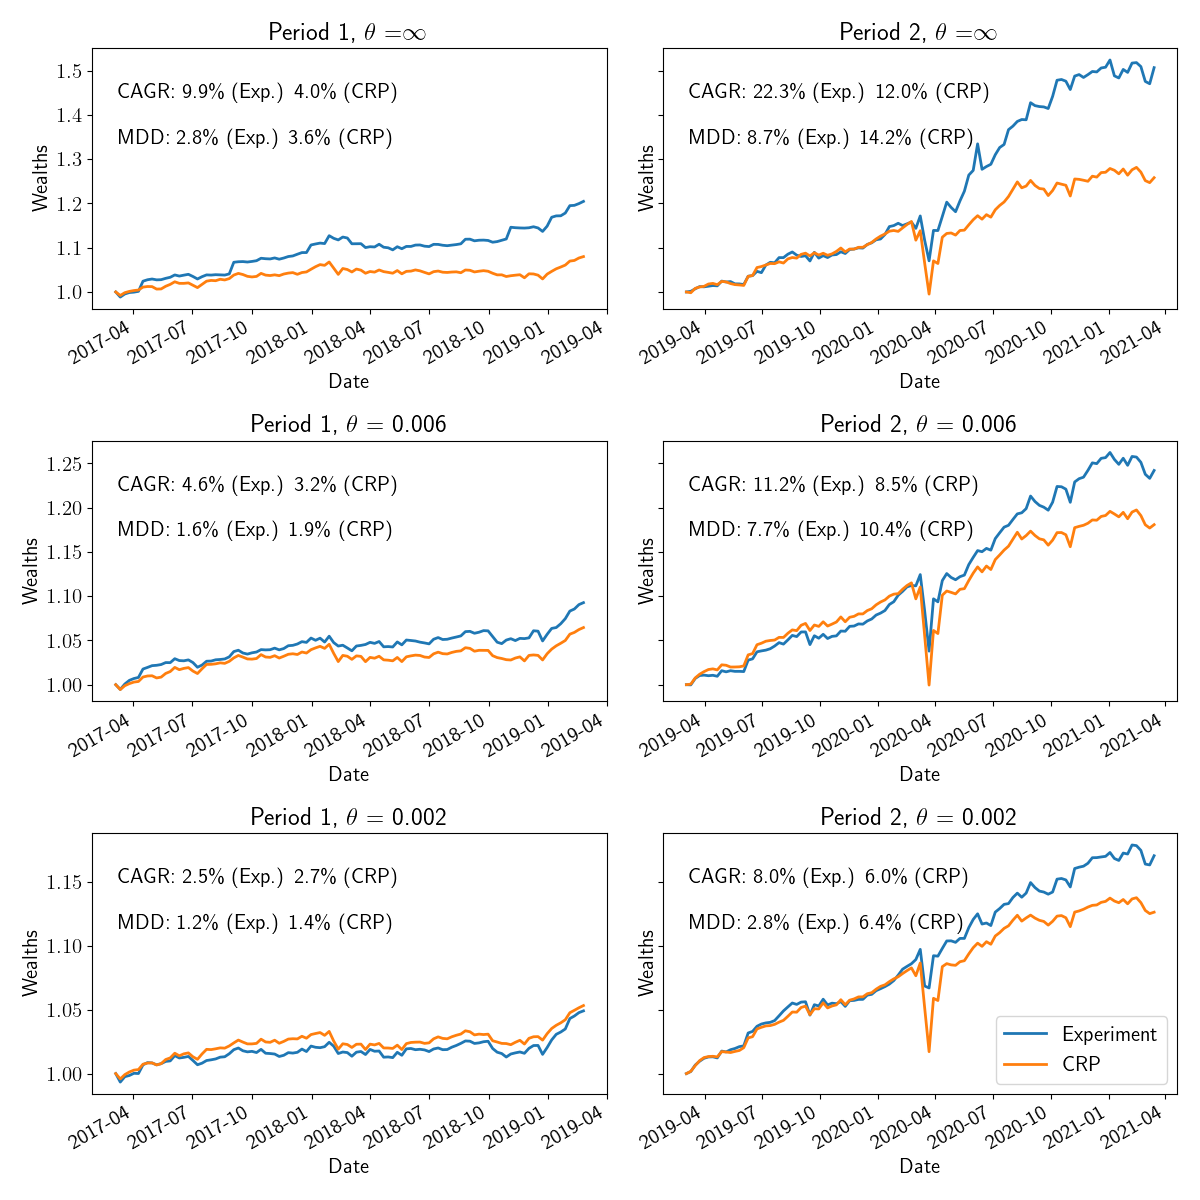
\includegraphics[width=15cm]{images/crp_compare.png}
  \caption [Comparison of experiments result with CRP]{Comparison of experiments result with CRP}
  \label{fig:crp_compare}
\end{figure}